\documentclass{beamer}

\mode<presentation> {

  \usetheme{Boadilla}
  \usecolortheme{dolphin}
  % \setbeamertemplate{footline}
  \setbeamercovered{transparent}

  \AtBeginSection[]{
  \begin{frame}
  \vfill
  \centering
  \begin{beamercolorbox}[sep=8pt,center,shadow=true,rounded=true]{title}
    \usebeamerfont{title}\insertsectionhead\par
  \end{beamercolorbox}
  \vfill
  \end{frame}
}

}

\usepackage[utf8]{inputenc}
\usepackage[T1]{fontenc}
\usepackage[USenglish]{babel}
\usepackage[style=authoryear, backend=bibtex]{biblatex} 
   \bibliography{bibliography} 
   \usepackage{eurosym}
   \usepackage{booktabs}
\usepackage{subfig}

\title{Convergence clubs and trees}
\author{Nikolas, Philipp, Lukas \& Daniel}
\date{6 December 2018}

\begin{document}

\begin{frame}[plain]
  \titlepage
  \begin{center}
   \textcite{postiglione2010regression} \\
   \citetitle{postiglione2010regression} \\
  \end{center}
\end{frame}

%%%%%%%%%%%%%%%%%%%%%%%%%%%%%%
% Presentation should cover: %
% - Research Question        %
% - Data                     %
% - Model specification      %
%%%%%%%%%%%%%%%%%%%%%%%%%%%%%%

\begin{frame}
  \frametitle{Introduction}
  \begin{itemize}
  \item Persistent country differences in GDP per capita\footnotemark
  \item Hypothesis: convergence within clubs but not inbetween
  \item Concept of $\beta$-convergence:
    $$
    ln(y_t / y_0) = \alpha + \beta ln(y_0) + \varepsilon_t, \quad \varepsilon_t \sim N(0, \sigma_\varepsilon^2 I)
    $$
  \item Spatial dependence likely\footnotemark
  \end{itemize}
  \footnotetext[1]{\cite{barro1995economic}}
  \footnotetext[2]{\cite{anselin1988lagrange}}
\end{frame}

\begin{frame}
  \frametitle{Regional convergence}
  \begin{itemize}
  \item Consider spatial correlation or heterogeneity
  \item Filtered SAR-reformulation: 
    $$
    (I_n - \rho W) ln(y_t/y_0) = \alpha + \beta ln(y_0) + \omega_t, \quad \omega_t \sim N(0, \sigma_\omega^2 I)
    $$
  \item Filtered SEM-reformulation: 
    $$
    (I_n -\delta W) ln(y_t/y_0) = \alpha + \beta \left[(I-\rho W) ln(y_0)\right] + u_t, \quad u_t \sim N(0, \sigma_u^2 I)
    $$
  % \item SDM?
  \end{itemize}
\end{frame}

\begin{frame}
  \frametitle{Club identification}
  \begin{itemize}
  \item Generally two different approaches:
    \begin{enumerate}
    \item Select countries based on \emph{a priori} criteria (e.g. GDP level)
    \item Consider the number of clubs as endogenous
    \end{enumerate}
  \end{itemize}
  \begin{block}{A regression tree algorithm}
    \begin{itemize}
    \item Non-parametric method to determine clubs
    \item Separate data using control variables
    \item Objective: find regions with similar coefficients 
    \end{itemize}
  \end{block}
\end{frame}

\begin{frame}
  \frametitle{Regression trees}
  \begin{itemize}
  \item Utilise binary recursive partitioning to subdivide a dataset
  \item Splits determined by imposed linear conditions on covariates
  \item In this case:
    \begin{itemize}
    \item Find regions with similar parameters 
    \item Split if coefficients within clubs are significantly different
    \end{itemize}
  \end{itemize}
\end{frame}

\begin{frame}
  \frametitle{The algorithm}
  \begin{itemize}
  \item Let $Z$ be the splitting variables, with $z_{i, j}$ as variable $i$ in region $j$
  \end{itemize}
    \begin{block}{The algorithm}
      \begin{enumerate}
        \setcounter{enumi}{-1}
      \item Start by estimating a pooled model for all EU regions \\
      \vspace{1em} At each step $k$, for each club $C$ in the set of clubs $S_k$:
      \item For every $z_i$ partition the club s.t. $z_{i, j} > z_{i, curr}$ and $z_{i, j} \leq z_{i, curr}$
        \begin{itemize}
        \item Re-estimate the model
        \item Determine if the coefficients are significantly different
        \end{itemize}
      \item Use the best split (smallest p-value) for the next set of clubs $S_{k+1}$
      \item End if:
        \begin{itemize}
        \item No more significant differences
        \item Minimum club size is reached
        \item Maximum number of clubs is reached
        \end{itemize}
    \end{enumerate}
  \end{block}
\end{frame}

\begin{frame}
  \frametitle{Tree results}
  \centering
  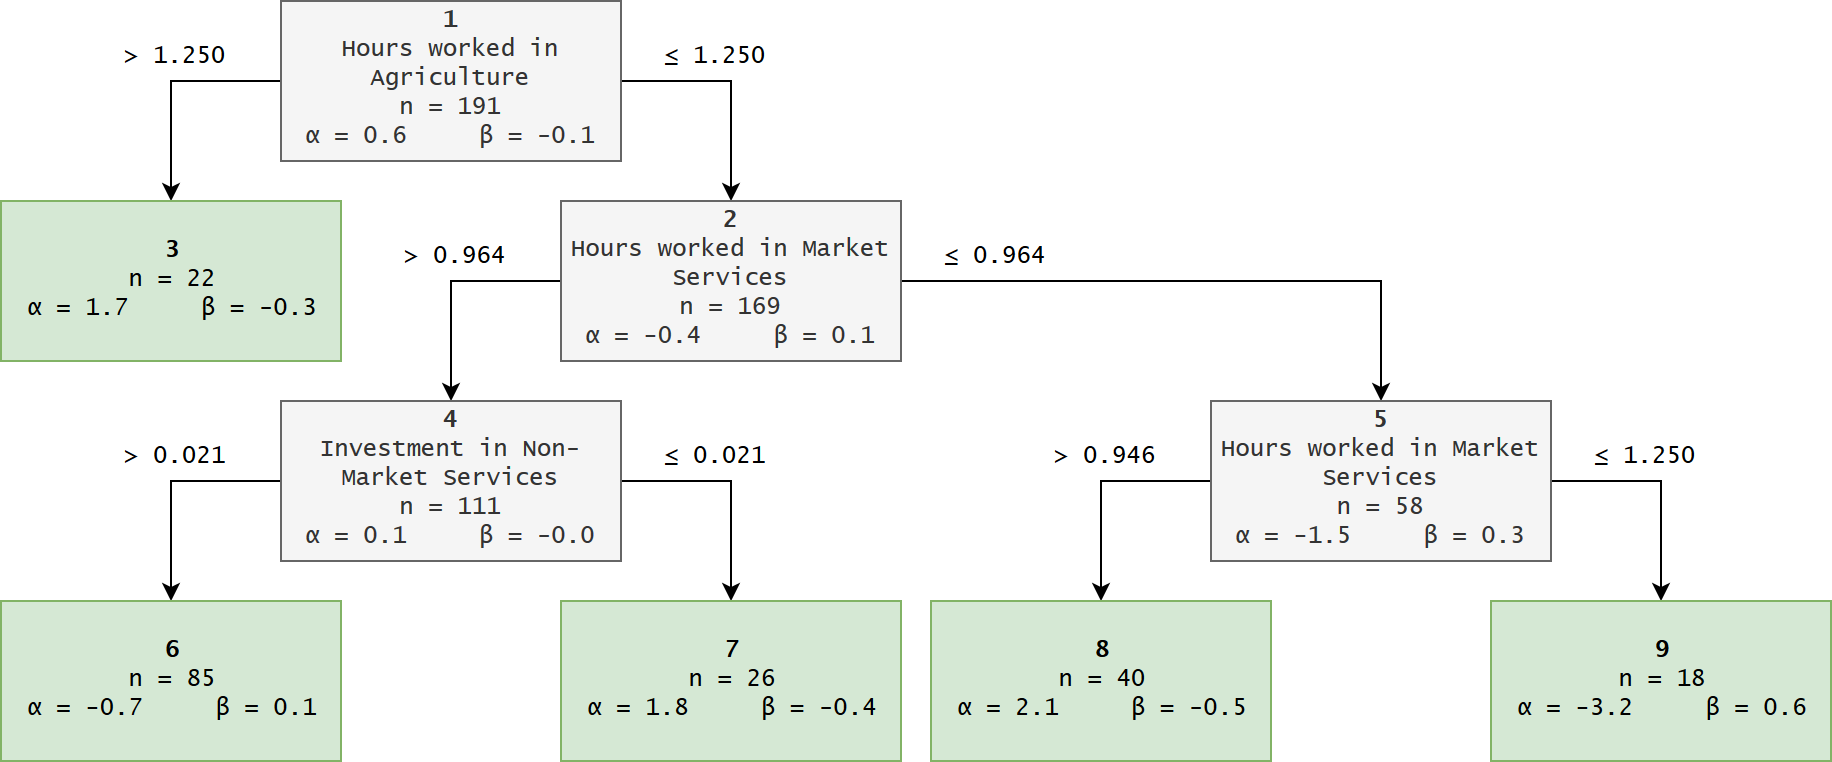
\includegraphics[width=12cm]{tree.png}
\end{frame}


\begin{frame}
  \frametitle{Data}
  \begin{itemize}
  \item Data obtained from European Regional Database by Cambridge Econometrics
  \item Timespan from 1980-2015; however, some regions only available from 1990 or 1995
  \item NUTS3 data only for certain indicators available - NUTS2 for all (NUTS2013)
  \item Available for 272 regions - yet to be determined if all will be included
  \item Data available for:
    \begin{itemize}
    \item GVA, GDP 
    \item Employment indicators (total hours worked, compensation etc.)
    \item Gross fixed capital formation
    \item Population
    \end{itemize}
  \end{itemize}
\end{frame}

\begin{frame}
  \frametitle{Data Inspection}
  \begin{figure}%
    \centering
    \subfloat[Initial income levels]{{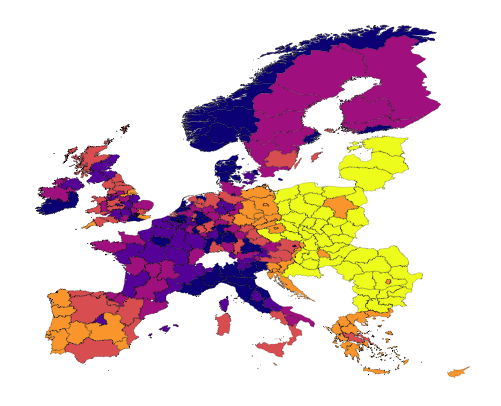
\includegraphics[width=5cm]{gva96.png} }}%
    \qquad
    \subfloat[Income growth rates]{{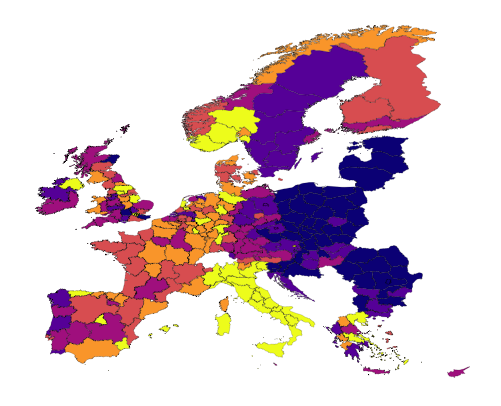
\includegraphics[width=5cm]{gr96_14.png} }}%
    \caption{Quantile maps of initial level of income and subsequent growth rates}%
    \label{fig:quantile}%
  \end{figure}
\end{frame}

\begin{frame}
  \frametitle{Spatial Dependence}
  \begin{figure}%
    \centering
    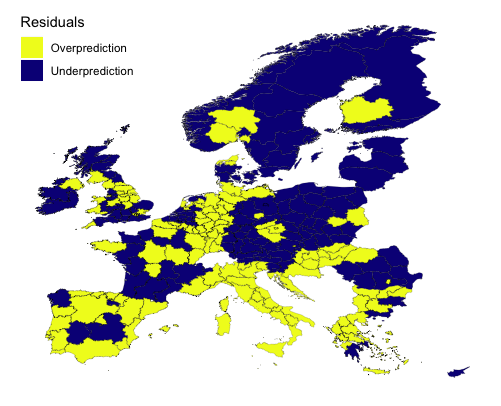
\includegraphics[width=7cm]{residuals_OLS.png}
    \caption{Map of OLS residuals with no club specification}%
    \label{fig:residuals}%
  \end{figure}
\end{frame}



\begin{frame}[allowframebreaks]
  \frametitle{References}
  \printbibliography
\end{frame}



\end{document}